% !TeX root = principal.tex
\documentclass{report}

\usepackage[brazil]{babel}
\usepackage[dvips]{epsfig}
\usepackage{graphicx,color}

\usepackage{lscape, rotating}
\usepackage{varioref,float,amssymb,amsmath}
\usepackage{float,amsfonts,amsthm}
\usepackage{changebar,longtable}
\usepackage[utf8]{inputenc}
\usepackage[T1]{fontenc}
\usepackage{fancyhdr}
\usepackage{makeidx}
%\makeindex
\usepackage[numbers]{natbib} 
%\usepackage{draftcopy}
\usepackage{subfigure}
%\draftcopySetGrey{.98}
\newcommand{\B}{{\tt\symbol{92}}}
\newcommand{\til}{{\tt\symbol{126}}}
\newcommand{\chap}{{\tt\symbol{94}}}
\newcommand{\agud}{{\tt\symbol{13}}}
\newcommand{\crav}{{\tt\symbol{18}}}
\newcommand{\cat}[3]{#1 \stackrel{#2}{\mathbf{\sqcap}}#3}

\newtheorem{lema}{Lema}%[section]
\newtheorem{teore}{Teorema}%[section]
\newtheorem{defi}{Definição}%[section]
\newtheorem{corol}{Corolário}%[section]
\newtheorem{ex}{Exemplo}%[section]
\newtheorem{propri}{Propriedade}%[section]
\newcommand{\dem}{\noindent \underline{Demonstração}: $\,$}
\newcommand{\fim}{\hfill $\rule{2.0mm}{2.0mm}$ \\}    % marcação de fim das demonstrações

%\renewcommand{\sectionmark}[1]{\markright{\thesection\ #1}}

\newtheorem{obs}{Observa\c{c}\~ao}%[section]
\newcommand{\preca}{pre\-con\-di\-ci\-o\-na\-da}
\newcommand{\preco}{pre\-con\-di\-ci\-o\-na\-do}
\newcommand{\precor}{pre\-con\-di\-ci\-o\-na\-dor}
\newcommand{\precors}{pre\-con\-di\-ci\-o\-na\-do\-res}
\newcommand{\bibdirec}{C:}
\newcommand{\range}[1]{\ensuremath{\operatorname{Im}(#1)}}
\newcommand{\Ker}[1]{\ensuremath{\operatorname{Nuc}(#1)}}
\newcommand{\dime}[1]{\ensuremath{\operatorname{dim}(#1)}}
\newcommand{\norma}[1]{\ensuremath{{\Vert #1\Vert}}}
\newcommand{\gera}[1]{\ensuremath{{\langle #1\rangle}}}
\newcommand{\bml}{\ensuremath{\mathbf{b}}}
\newcommand{\xml}{\ensuremath{\mathbf{x}}}
\newcommand{\yml}{\ensuremath{\mathbf{y}}}
\newcommand{\rml}{\ensuremath{\mathbf{r}}}
\newcommand{\hml}{\ensuremath{\mathbf{h}}}
\newcommand{\bbox}{\ensuremath{\mathcal{B}_n^{\Box}}}
\newcommand{\bboxo}{\ensuremath{\mathcal{\overline{B}}_n^{\Box}}}

%\newcommand{\versao}[2]{\ifthenelse{\boolean{versaocnmac}}{#1}{#2}}
\newcommand{\oblq}{%
 \ensuremath{%
   \mathrel{%
     \raisebox{-2.7pt}{$\scriptstyle-$}%
     \hspace{-4.5pt}%
     \raisebox{0.1pt}{$\scriptscriptstyle\not$}%
     \hspace{5.5pt}}}}

\newcounter{exernum}\setcounter{exernum}{0}
\newcounter{totexernum}
\newcounter{equaux}%for numbering equations
%introducao dos pacotes abaixo

\usepackage{calc}
\usepackage{subfigure}
\usepackage{ifthen}

\renewcommand\theequation{\arabic{equation}}

\usepackage{float}
\floatstyle{ruled}
\newfloat{algor}{thp}{loa}%[section]
\floatname{algor}{Algoritmo}

%\setlength{\parindent}{1em} % Change the value as needed
% fim de introdução de novos pacotes

\title{Arnoldi, FOM, GMRES, Pares de Ritz e Pares Harmônicos de Ritz}
\author{ Luiz Mariano  Carvalho }

\date{\today
}

\begin{document}
	
\maketitle



Há uma unanimidade entre os pesquisadores da área de métodos iterativos para solução de sistemas lineares: não existe o melhor método para a solução de problemas com matrizes não-simétricas~\cite{NachtigalReddyEtAl1992How}. Outro ponto de vista comum é o de que, para matrizes não-normais, há muito ainda o  que se trabalhar na compreensão dos fatores que influenciam na convergência dos mêtodos. Ainda outro consenso, é o da necessidade de precondicionadores para acelerar os métodos de projeção em subespaços de Krylov (MPSK). Na Seção \ref{arnol_sec_arnol}, o método de Arnoldi,  um dos procedimentos seminais dos MPSK ao lado do método de Lanczos, é discutido a partir de uma motivação para a sua construção e várias de suas propriedades são relacionadas. Nas demais seções, discutimos dois métodos paradigmáticos: o FOM e o GMRES. A literatura sobre esses métodos é vasta, estando consolidada, por exemplo, nos livros \cite{Brezinski2002Outils}, \cite{Greenbaum97Iterative}, \cite{Saad03Iterative},  \cite{Vorst03Iterative}.  Ao fim deste trabalho, tocamos levemente na questão de estabilidade do GMRES quando do uso  do procedimento de Arnoldi baseado no método de reflexões de Householder ou no método de ortogonalização de Gram-Schmidt modificado,  apresentando a bibliografia necessária ao estudo desse tema. 

\section{Método de Arnoldi}\label{arnol_sec_arnol}
O nome de Arnoldi\footnote{Walter Edwin Arnoldi (1917-1995) foi um engenheiro americano que publicou sua técnica em 1951, não muito distante do aparecimento do algoritmo de Lanczos. Arnoldi graduou-se em engenharia mecânica no Stevens Institute of Technology, Hoboken, New
Jersey, em 1937 e o seu mestrado foi obtido na Harvard University em 1939. Durante sua carreira, trabalhou como engenheiro na Hamilton Standard Division da United Aircraft Corporation, aonde, com o passar do tempo, tornou-se pesquisador chefe da divisão. Aposentou-se em 1977. Apesar de sua pesquisa ter versado sobre propriedades mecânicas e aerodinâmicas de aeronaves e estruturas aeroespaciais, o nome de Arnoldi é mantido vivo graças ao seu procedimento de ortogonalização (traduzido de \cite{Meyer00Matrix}).} aparece tanto ligado à solução de problemas de autovalores quanto à solução de sistemas lineares.  Apresentaremos o método de Arnoldi \cite{Arnoldi51principle} para ortogonalizar uma base de um subespaço Krylov.
 Visando facilitar o desenvolvimento, vamos supor que o grau do polinômio mínimo  de $r_0$ em relação a $A$ é maior do que $k$.

Uma motivação interessante para o método de Arnoldi é apresentada em \cite[pág. 337]{Meurant1999Computer} e foi formulada originalmente por Kees Vuik. Queremos construir uma base ortonormal para $\mathcal{K}_k(A,r_0)$ $=\gera{r_0,Ar_0,\ldots,A^{k-1}r_0}$, tal que $\mathcal{K}_k(A,r_0)$ $=\gera{v_1,v_2,\ldots,v_{k-1},v_k}$. Seja $V=\begin{pmatrix}v_1&v_2&\ldots &v_k\end{pmatrix}$, logo $V^HV=I$. Vale, também, observar que a matriz de Krylov  associada a $\mathcal{K}_k(A,r_0)$, ${K}_k=\begin{pmatrix} r_0&Ar_0&\ldots&A^{k-1}r_0\end{pmatrix}$, goza da seguinte propriedade:
\begin{gather}
A{K}_k=\begin{pmatrix} Ar_0&A^2r_0&\ldots&A^kr_0\end{pmatrix}=\notag\\
=\begin{pmatrix} Ar_0&A^2r_0&\ldots&A^{k-1}r_0&0\end{pmatrix} +\begin{pmatrix} 0&0&\ldots&A^kr_0\end{pmatrix}=\notag\\
={K}_k\begin{pmatrix}
0 & 0 & \ldots & 0 & 0 \\
1 & 0 & \ldots & 0 & 0  \\
0 & 1& \ddots & \vdots & \vdots\\
\vdots & \vdots & \ddots & 0 & 0\\
0 & \ldots & \ldots & 1 & 0 \\
\end{pmatrix}+A^kr_0e_k^H. \label{eq_arnoldi_krylhesse}
\end{gather}
onde $e_k$ é o $k$-ésimo vetor da base canônica. Como buscamos uma base ortonormal, o método usual é o da fatoração ${K}_k=QR$, onde $Q$ é uma matriz $m\times k$, cujas colunas são vetores ortonormais, e $R$ é uma matriz não singular e triangular superior. Chamando de $H_1$ a matriz de Hessenberg que aparece em \eqref{eq_arnoldi_krylhesse}, teremos
\[AQR=QRH_1+A^kr_0e_k^H.\]
Mais algumas contas:

\begin{multline*}
AQ=(QRH_1+A^kr_0e_k^H)R^{-1}\Rightarrow Q^HAQ=(RH_1+Q^HA^kr_0e_k^H)R^{-1}\Rightarrow\\
\Rightarrow Q^HAQ=R(H_1+R^{-1}Q^HA^kr_0e_k^H)R^{-1},
\end{multline*}
ora
\[H_2:=H_1+R^{-1}Q^HA^kr_0e_k^H=\begin{pmatrix}
    0 & 0 & \ldots & 0 & \vdots \\
     1 & 0 & \ldots & 0 & \vdots  \\
     0 & 1& \ddots & \vdots & R^{-1}Q^HA^kr_0 \\
     \vdots & \vdots & \ddots & 0 & \vdots\\
     0 & \ldots & \ldots & 1 & \vdots \\
     \end{pmatrix},\]
     é uma matriz de Hessenberg e $RH_2R^{-1}$ também o será. E assim, vemos que a decomposição $Q^HAQ$ é uma matriz de Hessenberg superior. E, podemos tomar para $V$ as colunas de $Q$.

%\ifthenelse{\boolean{versaocnmac}}{}
{
     Avancemos  com o raciocínio de Vuik. Vamos desenvolver a  última  coluna de $RH_2R^{-1}$.
     Ela será  igual a $Q^HA^kr_0R^{-1}(k,k)$, para isso bastando interpretar a multiplicação de matrizes como um produto externo.  $R^{-1}(k,k)$ é igual a $1/\norma{\widetilde{Q}(:,k)}_2$, onde $\widetilde{Q}(:,k)$ é o vetor ${Q}(:,k)$ antes da normalização, ou seja, ${Q}(:,k)=\widetilde{Q}(:,k)/\norma{\widetilde{Q}(:,k)}_2$. E assim, comparando as  última s colunas das matrizes $Q^HAQ$ e $RH_2R^{-1}$, temos
     \[
     Q^HA{Q}(:,k)=Q^HA^kr_0/\norma{\widetilde{Q}(:,k)}_2,
     \]
     ou ainda
     \[QQ^HA\widetilde{Q}(:,k)=QQ^HA^kr_0.\]
     Ou seja, as projeções ortogonais de $A\widetilde{Q}(:,k)$ e de $A^kr_0$ no subespaço de Krylov $\mathcal{K}_k(A,r_0)$ são  as mesmas. não temos ainda a resposta final, mas uma boa pista, de como gerar os subespaço de Krylov sem utilizar $A^kr_0$. Será que no processo de ortogonalização, ao substituirmos  o vetor $A^kr_0$ pelo vetor $A\widetilde{Q}(:,k)$, estaremos gerando bases para o mesmo subespaço de Krylov $\mathcal{K}_k(A,r_0)$? Quais as condições sobre os vetores $A^kr_0$ e $A\widetilde{Q}(:,k)$ para que os subespaços gerados sejam os mesmos? A resposta positiva é o método de Arnoldi que está descrito nos Algoritmos \ref{algor_arnoldigs} e \ref{algor_arnoldigsm}.
}
     \begin{algor}[htb]
\caption{ Método  de Arnoldi $(A,\;r_0,\;k)$ - alternativa com Gram-Schmidt clássico.} \label{algor_arnoldigs}

{%\footnotesize
\begin{enumerate}
\renewcommand{\labelenumi}{\theenumi:}
\setlength{\itemsep}{.01cm}
\item $V(:,1)=r_0/\norma{r_0}$
\item para $j=1:k$
\item~~~$w=AV(:,j)$
\item~~~$H(1:j,j)=V(:,1:j)^Hw$
\item~~~$w=(I-V(:,1:j)V(:,1:j)^H)w$
\item~~~$H(j+1,j)=\norma{w}_2$
\item~~~$V(:,j+1)=w/H(j+1,j)$
\item fim-para
\renewcommand{\labelenumi}{\theenumi.}
\end{enumerate}
}
\end{algor}
O Algoritmo \ref{algor_arnoldigs} usa o processo de ortogonalização de Gram-Schmidt clássico, onde todos os escalares  utilizados para multiplicar os elementos da base já  existente são  calculados usando o mesmo valor de $w=AV(:,j)$. Esse procedimento é numericamente instável, e por razões de estabilidade uma versão  modificada é utilizada \cite{Stewart1973Introduction}\footnote{Para ver exemplo de instabilidade consultar, entre outros, \cite[exemplo 5.5.5, pág. 316]{Meyer00Matrix}.}, ver Algoritmo \ref{algor_arnoldigsm}.
     \begin{algor}[htb]
\caption{ Método  de Arnoldi $(A,\;r_0,\;k)$  - alternativa com  Gram-Schmidt modificado.}\label{algor_arnoldigsm}

  {%\footnotesize
\begin{enumerate}
\renewcommand{\labelenumi}{\theenumi:}
\setlength{\itemsep}{.01cm}
\item $V(:,1)=r_0/\norma{r_0}_2$
\item para $j=1:k$
\item\label{algor_arnoldigsm_it_wav}~~~$w=AV(:,j)$
\item~~~para $i=1:j$
\item~~~~~~$H(i,j)=(V(:,i),w)$
\item~~~~~~$w=w-H(i,j)V(:,i)$
\item~~~fim-para
\item\label{algor_arnoldigsm_hj1j}~~~$H(j+1,j)=\norma{w}_2$
\item\label{algor_arnoldigsm_vj1}~~~$V(:,j+1)=w/H(j+1,j)$
\item fim-para
\renewcommand{\labelenumi}{\theenumi.}
\end{enumerate}
}
\end{algor}
\begin{obs}\label{obs_arnoldiruptura}
Em ambas as versões do algoritmo de Arnoldi ainda não há um teste  sobre  $H(j+1,j)$ ser numericamente zero (ou seja, menor que uma constante arbitrada). Esse fato, denominado de \textbf{ruptura} do algoritmo, ocorre quando o novo vetor pertence em precisão finita ao mesmo subespaço dos vetores  gerados  até  aquele momento. Ou seja, quando $\mathcal{K}_k(A,r_0)\supset A\mathcal{K}_k(A,r_0)$ ou, ainda, $\mathcal{K}_k(A,r_0)= \mathcal{K}_{k+1}(A,r_0)$. Em uma real implementação computacional é necessária a inclusão  de um teste de ruptura.
\end{obs}
\begin{obs}\label{obs_mgsgsdif}
Em \cite[pág. 279]{Stewart98Matrix}, o autor é bastante enfático quanto a inadequação do nome Gram-Schmidt modificado, uma vez que ele considera ser outro método com outras propriedades apesar da semelhança entre os algoritmos, para maiores detalhes ver a obra citada.
\end{obs}
Sejam $V_k\in\mathbb{C}^{m\times k}$, a matriz cujas colunas são  os vetores $V(:,j)$, e $H_k\in\mathbb{C}^{k\times k}$, a matriz Hessenberg superior, formadas no procedimento de Arnoldi  até  a $k$-ésima iteração do Algoritmo \ref{algor_arnoldigsm} antes de executarmos os passos \ref{algor_arnoldigsm_hj1j}: e \ref{algor_arnoldigsm_vj1}:. O algoritmo completo, contadas as $k$ iterações, terá uma representação matricial,  até  esse momento, dada por
\begin{equation}\label{arnol_prop_avk-vkhwekh}
AV_k-V_kH_k=we_k^H,
\end{equation}
onde $e_k$ é o $k$-ésimo vetor da base canônica. Ao incorporarmos os passos  \ref{algor_arnoldigsm_hj1j}: e \ref{algor_arnoldigsm_vj1}:, passamos a ter:

\begin{gather}
AV_k-V_kH_k=H(k+1,k)V(:,k+1)e_k^H \Rightarrow \notag\\ \Rightarrow AV_k=V_kH_k+H(k+1,k)V(:,k+1)e_k^H\label{arnol_prop_soma}.
\end{gather}
Temos aqui uma multiplicação entre matrizes representada por um produto externo e podemos escrevê-la de forma mais compacta como:
\begin{equation}\label{arnol_prop_comple}
AV_k=V_{k+1}\overline{H}_k,
\end{equation}
onde $V_{k+1}\in\mathbb{C}^{m\times (k+1)}$ e $\overline{H}_k\in\mathbb{C}^{(k+1)\times k}$.
Há, ainda, uma relação simples a ser extraída:
\begin{equation}\label{arnol_prop_hk}
V_k^HAV_k={H}_k.
\end{equation}



 As fórmulas \eqref{arnol_prop_soma}, \eqref{arnol_prop_comple} e \eqref{arnol_prop_hk} resumem algumas das propriedades do método de Arnoldi que usaremos adiante.

 \begin{obs}\label{arnol_obs_vkavk}
 Vale observar que a fórmula \eqref{arnol_prop_hk} nos lembra  a decomposição de Schur (só que na decomposição de Schur, $V_k$ é, necessariamente, quadrada), ver ~\cite[pág. 79]{HornJohnson1985}. E, motivados por essa observação, podemos utilizar autovalores relacionados à matriz ${H}_k$ visando aumentar a velocidade de convergência dos  métodos de Krylov baseados no procedimento de Arnoldi.
 \end{obs}

\section{Ortogonalização Completa - FOM}\label{arnol_sec_fom}

Para resolver $Ax=b$, o método da \textbf{ortogonalização completa}~\cite{Saad1981Krylov}, \cite{Saad03Iterative} é um MPSK com as seguintes características:  partindo de um valor inicial $x_0$, tem-se o  resíduo inicial, $r_0=b-Ax_0$. $\mathcal{K}_k$ será o subespaço de Krylov $\mathcal{K}_k(A,r_0)$. A cada nova iteração, calcula-se $x_k$  impondo as condições: $(x_k-x_0)\in \mathcal{K}_k(A,r_0)$ e o  resíduo $r_k=b-Ax_k$ deve ser ortogonal à $\mathcal{L}_k=\mathcal{K}_k(A,r_0)$. Nesse caso, o espaço de restrições será $\mathcal{L}_k=\mathcal{K}_k$ e $r_k\perp \mathcal{K}_k(A,r_0)$. Uma representação gráfica simplificada desse fato pode ser vista na figura \ref{fig_kryakrybfom}.

\begin{figure}[htb]
  % Requires \usepackage{graphicx}
  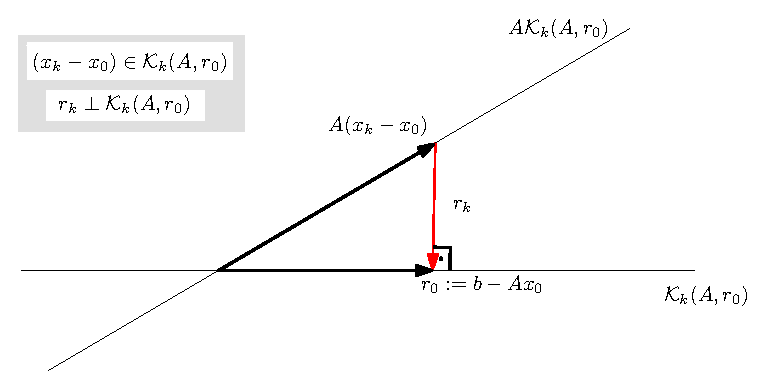
\epsfig{file=arnol_fom.eps, width=\linewidth}
  \caption{Representação esquemática da condição de ortogonalidade do  resíduo do FOM.}\label{fig_kryakrybfom}
\end{figure}

Uma representação resumida da estrutura de uma iteração do FOM é apresentada no Algoritmo \ref{algor_fomesquema}.
     \begin{algor}[htb]
\caption{Ortogonalização completa $(A,\;x_0)$ - resumo de uma iteração}\label{algor_fomesquema}
{%\footnotesize
\begin{enumerate}
\renewcommand{\labelenumi}{\theenumi:}
\setlength{\itemsep}{.01cm}
\item\label{algor_fomesquema_arnoldi} adicionar um vetor a uma base ortonormal para o subespaço de Krylov $\mathcal{K}_j(A,r_0)$,
\item\label{algor_fomesquema_xjrj} calcular $x_j$ tal que $x_j-x_0\in \mathcal{K}_j(A,r_0)$ e que $r_j\perp \mathcal{K}_j(A,r_0)$.
\renewcommand{\labelenumi}{\theenumi.}
\end{enumerate}
}
\end{algor}
O primeiro passo do Algoritmo \ref{algor_fomesquema} será feito pelo método de Arnoldi. No segundo passo, as condições dadas nos permitem detalhar as operações matriciais necessárias. Seja $V_j$ uma base ortonormal para $\mathcal{K}_j(A,r_0)$, então temos que para algum $y_j\in\mathbb{C}^j$, $x_j-x_0=V_jy_j$, o que atende à primeira condição. Quanto ao  resíduo, ele tem que ser ortogonal ao mesmo espaço, ou seja $r_j^HV_j=0$ ou $V_j^Hr_j=0$, mas
\begin{multline*}
r_j=b-Ax_j=b-A(x_0+V_jy_j)=r_0-AV_jy_j\Rightarrow V_j^H(r_0-AV_jy_j)=0\Rightarrow \\ \Rightarrow V_j^HAV_jy_j=V_j^Hr_0 \Rightarrow H_jy_j=V_j^Hr_0.
\end{multline*}
Como essa base é ortonormal e o primeiro vetor da base é, exatamente, $r_0/\norma{r_0}_2$, então $V_j^Hr_0=\big((r_0/\norma{r_0}_2)^Hr_0,0,\ldots,0\big)$. Logo, temos que resolver o sistema
\[
H_jy_j=\norma{r_0}_2 e_1,
\]
onde $e_1$ é o primeiro vetor da base canônica de $\mathbb{C}^j$. Para que esse sistema tenha solução única é necessáro e suficiente que $H_j$ seja uma matriz não singular. Essa condição não será sempre garantida e a singularidade de $H_j$ pode ocorrer em duas situações distintas. No primeiro caso, será uma ruptura benéfica do algoritmo:
\[
H_jy_j=0\Rightarrow V_j^HAV_jy_j=0\Rightarrow V_j^HA\sum_{i=1}^j\alpha_iv_i=0,
\]
como as colunas de $V_j$ geram uma base para   $\mathcal{K}_j(A,r_0)$ temos ainda que
\[
V_j^HA\sum_{i=1}^j\alpha_iv_i=0\Rightarrow V_j^HA\sum_{i=1}^j\alpha_i\bigg(\sum_{k=1}^j\beta_k A^{k-1}r_0\bigg)=0,
\]
nesse caso, vamos considerar que $AV_jy_j=0$
\[
A\sum_{i=1}^j\alpha_i\bigg(\sum_{k=1}^j\beta_k A^{k-1}r_0\bigg)=0\Rightarrow \sum_{i=1}^j \gamma_i A^ir_0=0,
\]
ou seja chegamos ao polinômio mínimo de $r_0$ em relação a $A$ e temos a solução exata.

Mas outra situação também pode ocorrer, nesse caso $z_j:=AV_jy_j\neq 0$ e $V_j^Hz_j=0$, ou seja, existe um vetor não-nulo em $A\mathcal{K}_j(A,r_0)$ que é ortogonal a $\mathcal{K}_j(A,r_0)$, também nesse caso a matriz $H_j$ será singular e haverá uma ruptura do FOM, sem ser benéfica.

O próximo resultado mostra como o cálculo do  resíduo é simples para o FOM.

\begin{teore}
O  resíduo da $j$-ésima iteração do FOM é dado por

\[
r_j=-\overline{H}_j(j+1,j)V_{j+1}(:,(j+1)) e_j^T y_j \quad\text{e}\quad \norma{r_j}_2=\overline{H}_j(j+1,j)|e_j^T y_j|.
\]


\end{teore}
\dem
\begin{eqnarray*}
r_j&=&b-Ax_j=b-Ax_0-AV_jy_j=r_0-V_{j+1}\overline{H}_jy_j=\\
&=&r_0-(V_jH_j+\overline{H}_j(j+1,j)V_{j+1}(:,(j+1))e_j^T)y_j=\\
&=&\beta V_j e_1-(V_jH_j+\overline{H}_j(j+1,j)V_{j+1}(:,(j+1))e_j^T)y_j=\\
&=&V_j(\beta  e_1-H_jy_j)-\overline{H}_j(j+1,j)V_{j+1}(:,(j+1))e_j^T y_j=\\
&=&-\overline{H}_j(j+1,j)V_{j+1}(:,(j+1))e_j^T y_j.\\
\end{eqnarray*}
Como $\overline{H}_j(j+1,j)e_j^T y_j$ é um escalar e $\norma{V_{j+1}(:,(j+1))}_2=1$, temos os resultados.
\fim

\markboth{Arnoldi}{ Resíduo Minimal Generalizado - GMRES}

\section{Resíduo Minimal Generalizado - GMRES}\label{arnol_sec_gmres}
O método de \textbf{ resíduo minimal generalizado (GMRES)}~\cite{SaadSchultz86GMRES} é um MPSK com as seguintes características. Para resolvermos $Ax=b$, partimos de um valor inicial $x_0$ e  calculamos o  resíduo inicial, $r_0=b-Ax_0$. $\mathcal{K}_k$ será o subespaço de Krylov $\mathcal{K}_k(A,r_0)$, ou seja, $(x_k-x_0)\in \mathcal{K}_k(A,r_0)$, e o espaço de restrições será $\mathcal{L}_k=A\mathcal{K}_k(A,r_0)$ e, assim, o  resíduo $r_k$ é ortogonal a $A\mathcal{K}_k(A,r_0)$, $r_k\perp A\mathcal{K}_k(A,r_0)$. Com isso, o GMRES assegura que o  resíduo, a cada iteração, não aumentará, no pior caso o  resíduo  das novas iterações será igual ao(s) da(s) anterior(es). Como a cada passo o espaço de busca está aumentando, mesmo depois de alguma \textbf{estagnação}, o método encontrará um ponto melhor. Uma representação gráfica simplificada desse fato pode ser vista na figura \ref{fig_kryakrybgmres}.

\begin{figure}[htb]
  % Requires \usepackage{graphicx}
  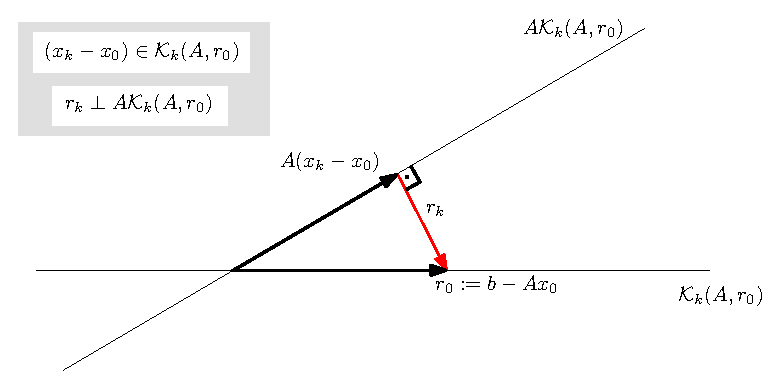
\epsfig{file=arnol_gmres.eps, width=\linewidth}
  \caption{Representação esquemática da condição de ortogonalidade do  resíduo do GMRES.}\label{fig_kryakrybgmres}
\end{figure}


     \begin{algor}[htb]
\caption{GMRES $(A,\;x_0)$ - resumo de uma iteração}\label{algor_gmresesquema}
{%\footnotesize
\begin{enumerate}
\renewcommand{\labelenumi}{\theenumi:}
\setlength{\itemsep}{.01cm}
\item\label{algor_gmresesquema_arnoldi} adicionar um vetor a uma base ortonormal para o subespaço de Krylov $\mathcal{K}_j(A,r_0)$,
\item\label{algor_gmresesquema_xjrj} calcular $x_j$ tal que $x_j-x_0\in \mathcal{K}_j(A,r_0)$ e que $r_j\perp A\mathcal{K}_j(A,r_0)$.
\renewcommand{\labelenumi}{\theenumi.}
\end{enumerate}
}
\end{algor}

Uma representação resumida da estrutura de uma  iteração do GMRES é apresentada no Algoritmo \ref{algor_gmresesquema}, aonde o passo \ref{algor_gmresesquema_arnoldi}: será realizado através do método de Arnoldi e no passo \ref{algor_gmresesquema_xjrj}: haverá a solução de um problema de quadrados mínimos através de uma fatoração $QR$ adequada.
Vejamos alguns dos detalhes desse processo:
\[
r_k=b-Ax_k=b-A(x_0+c_k)=r_0-Ac_k, \quad c_k\in\mathcal{K}_k(A,r_0);
\]
sejam $V_{k+1}$ uma matriz cujas colunas formam uma base ortonormal  para $\mathcal{K}_{k+1}(A,r_0)$ e $V_k$ uma matriz cujas colunas formam uma base ortonormal  para $\mathcal{K}_k(A,r_0)$, então $c_k=V_k y_k$, $y_k\in\mathbb{C}^k$, e podemos continuar o desenvolvimento acima,  lembrando-nos de uma das relações de Arnoldi, $AV_k=V_{k+1}\overline{H}_k$:
\[
r_k=r_0-Ac_k=r_0-AV_ky_k=r_0-V_{k+1}\overline{H}_ky_k.
\]
Na construção da base ortonormal consideramos $v_1=r_0/\norma{r_0}_2$, logo
\[
r_0-V_{k+1}\overline{H}_ky_k=\norma{r_0}_2v_1-V_{k+1}\overline{H}_ky_k=\norma{r_0}_2V_{k+1}e_1-V_{k+1}\overline{H}_ky_k
\]
temos, então
\[
r_k=V_{k+1}(\norma{r_0}_2e_1-\overline{H}_ky_k),
\]
 mas $\norma{V_{k+1}}_2=1$, uma vez que as suas colunas são  vetores ortonormais, logo o problema de quadrados mínimos que temos que resolver é
\begin{equation}\label{eq_gmresquadmin}
\norma{r_k}_2=\underset{y_k\in \mathbb{C}^k}{\min}\norma{\norma{r_0}_2e_1-\overline{H}_ky_k}_2.
\end{equation}

Desenvolvendo \eqref{eq_gmresquadmin}. Podemos construir o produto matricial \begin{equation}\label{eq_gmresquadminnovoproduto}
\norma{\begin{pmatrix}\overline{H}_k & \norma{r_0}_2e_1\\\end{pmatrix}\begin{pmatrix}
                                                                  y_k \\
                                                                  -1 \\
                                                                \end{pmatrix}}_2.
\end{equation}
Fazendo a fatoração $QR$ de \[
\begin{pmatrix}\overline{H}_k & \norma{r_0}_2e_1\\\end{pmatrix}=Q_{k+1}R_{k+1}= Q_{k+1} \begin{pmatrix}R_k & \zeta\\0 & s\end{pmatrix}.
       \]
E \eqref{eq_gmresquadminnovoproduto} pode ser escrita como:
\begin{equation}\label{eq_gmresquadminnovoprodutosemqk1}
\norma{ Q_{k+1}\begin{pmatrix}R_k & \zeta\\0 & s\end{pmatrix} \begin{pmatrix}y_k \\ -1 \\  \end{pmatrix}}_2=\norma{ \begin{pmatrix}R_k & \zeta\\0 & s\end{pmatrix} \begin{pmatrix}y_k \\ -1 \\  \end{pmatrix}}_2.
\end{equation}
Logo a expressão  \eqref{eq_gmresquadmin}, transforma-se em
\begin{equation}\label{eq_gmresquadminnovamin}
\norma{r_k}_2=\underset{y_k\in \mathbb{C}^k}{\min}\norma{\begin{pmatrix}R_k y_k-\zeta \\ s  \end{pmatrix}}_2= |s|.
\end{equation}
O que fornece uma forma simples\label{arnol_calcuresid} de se calcular a norma do  resíduo, pelo menos em aritmética exata (ou infinita). Essa informação será útil tanto para detectar a convergência do método como para observar algum processo de estagnação\footnote{No entanto \label{arnol_calcuresidprob} um alerta deve ser feito aqui, pois esse cálculo, quando feito em aritmética  finita, pode levar a  erro, uma vez que a igualdade pode não estar garantida, para maiores esclarecimentos desse fenômeno consultar \cite[pág. 90]{Chaitin-ChatelinFraysse1996Lectures}.}.

Relembrando a observação \ref{obs_arnoldiruptura}, haverá um momento em que $H(k+1,k)=0$, isso significa que  o novo vetor calculado pertence ao espaço de Krylov anterior ou seja $w\in\mathcal{K}_k(A,r_0)$, confira o Algoritmo \ref{algor_arnoldigsm}. 

A implementação do GMRES baseia-se na utilização de rotações de Givens para resolver o problema de quadrados mínimos. Como $\overline{H}_k$ é uma matriz de Hessenberg superior, as rotações são  utilizadas para anular todos os valores que se encontram exatamente abaixo da diagonal principal. As rotações atuam apenas em uma entrada por vez, o trabalho feito anteriormente é aproveitado, sendo uma alternativa atraente por sua economia e estabilidade.

No artigo inicial sobre o GMRES \cite{SaadSchultz86GMRES} foram apresentados resultados de convergência do método para matrizes normais. No entanto, segundo \cite{Vorst03Iterative}, o principal resultado sobre a convergência do GMRES para uma matriz qualquer é, no mínimo, intrigante e foi apresentado em \cite{GreenbaumPtakEtAl96Any}, em 1996.
\begin{teore}[Convergência do GMRES]\label{teo_gmresconverg}
Dada uma  sequência não crescente de reais positivos $f_0\ge f_1\ge\ldots \ge f_{m+1}$ e um conjunto de complexos não nulos $\lambda_1,\lambda_1,\ldots,\lambda_m$, então existe uma matriz $A$ com autovalores $\lambda_j$ e com lado direito $b=f_0e_1$ tal que os  resíduos $r_k$ do GMRES calculados na solução de $Ax=b$, com $x_0=0$, satisfazem $\norma{r_k}_2=f_k$, para $k=0:(n-1)$.
\end{teore}
\begin{obs}\label{obs_gmresconv}
O teorema \ref{teo_gmresconverg} nos informa que para uma matriz qualquer apenas os autovalores não são  suficientes para caracterizar o comportamento da convergência do GMRES. No entanto, para matrizes normais, os autovalores são  suficientes. também para matrizes bem condicionadas, mesmo que não normais, os autovalores dão informação sobre o a convergência do  método.
\end{obs}
\begin{obs}\label{obs_gmresconvcontraponto}
O outro lado da moeda do teorema \ref{teo_gmresconverg} é que, na prática, ele não influencia o uso ou não do GMRES, apenas dá uma informação sobre casos possíveis e não sobre casos que sempre ocorrerão. Um outro aspecto é que o GMRES tem, em muitos casos importantes, uma convergência lenta, necessitando de precondicionadores para funcionar em um número de iterações aceitável, nesse caso a informação fornecida pelo teorema não tem grande aplicação.
\end{obs}

 A discussão  sobre as ferramentas matemáticas para caracterização da convergência do GMRES, e dos demais  métodos de Krylov para matrizes não-normais, é uma área de estudo importante e que contém vários problemas em aberto, ver por exemplo \cite{Embree1999How},  \cite{PaigeParlettEtAl95Approximate}, \cite{SimonciniSzyld2007Recent}, \cite{Zemke2003Krylov}.

 Um comentário necessáro  é sobre a estabilidade do método GMRES. Há dois resultados em \cite{PaigeRozloznikEtAl2006MODIFIED} e \cite{Rozloznik1997Numerical} onde são  caracterizadas a estabilidade em relação ao erro inverso das implementações do GMRES usando as reflexões de Householder e o método modificado de Gram-Schmidt no processo de Arnoldi. Esses resultados asseguram que pequenas modificações nos dados tratados não irão acarretar grandes problemas é solução do problema, uma vez que se estará  resolvendo exatamente um problema próximo. Ou seja a dificuldade será  intrínseca ao prôprio sistema que está sendo resolvido e não devida ao algoritmo utilizado. Trata-se de uma leitura  técnica e importante para os pesquisadores da área.



A versão  utilizada na prática para o GMRES é a \textbf{com recomeço}. Com o avanço do número de iterações do GMRES, o armazenamento dos vetores necessáros e o tamanho dos problemas de quadrados mínimos a serem resolvidos começam a inviabilizar a aplicação do  método. Há várias alternativas: a escolha de um subconjunto reduzido dos vetores já  calculados  e o recomeço após de um número fixado de iterações (versões com recomeço). A versão  com recomeço padrão simplesmente testa a convergência depois de um número fixo de iterações  e, caso não se tenha atingido a cota desejada, mantêm-se apenas a  última  aproximação, descartando-se todos os demais vetores,  e usa-se esse aproximação como valor inicial para calcular um novo  resíduo inicial e  começar uma nova aplicação do GMRES\footnote{Cada ciclo completo de recomeço é denominado \textbf{ciclo} do GMRES.}, ver análises em \cite{Morgan95Restarted}, \cite{Simoncini00Convergence} e \cite{Trefethen1990Algorithms}. A vantagem dessa alternativa é que como cada iteração garante o não aumento da norma euclidiana do  resíduo, com o uso dessa solução, garante-se que estaremos partindo de um ponto, possivelmente melhor do que a primeira aproximação $x_0$. Apesar de  drástica, essa alternativa é das mais usadas na prática. A bem da verdade, a alternativa com recomeço é um método de Krylov apenas durante cada ciclo do GMRES, uma vez que a cada recomeço um novo subespaço de Krylov é construído, ou seja o método completo não fica dentro de um mesmo subespaço de Krylov que aumenta a cada ciclo completo.

Há dezenas de variantes do  GMRES que foram desenvolvidas nos últimos 20 anos, ver por exemplo \cite{SaadVorst00Iterative}, \cite{SimonciniSzyld2007Recent}, \cite{Zou2023}.



Discutiremos aproximações para autovalores das matrizes que aparecem durante a aplicação dos métodos iterativos para a solução dos sistemas lineares. Há uma vasta literatura sobre o tema, por exemplo \cite{Beattie1998Harmonic,GoossensRoose99Ritz,Morgan00Implicitly,PaigeParlettEtAl95Approximate,SleijpenVorst00JacobiDavidson}.

Vamos apresentar, inicialmente, uma abordagem feita em \cite{SleijpenEshof2003use}, onde se considera que o \textbf{método
de Rayleigh-Ritz}
é o melhor para uma boa aproximação em  um dado subespaço de  autovalores de uma matriz real e simétrica. Baseando-se em \cite[seção 11.4]{Parlett1998symmetric}, os autores dizem que esse método comporta-se bem para o cálculo de autovalores exteriores e seus autovetores associados, mas que, no entanto, o mesmo não ocorre para autovalores interiores ao espectro da matriz \cite{JiaStewart2001analysis,Morgan1991Computing,Scott1982Advantages}. Há estudos para se tentar ultrapassar os problemas com o cálculo dos autopares interiores e os autores citam os esforços feitos em \cite{Scott1982Advantages} e, em particular, em \cite{Morgan1991Computing}, aonde a inversão do operador (no nosso caso da matriz) pode ser tratada implicitamente (veremos como, no Teorema \ref{teo_SleijpenVorst00JacobiDavidson}).  A proposta recebeu o nome de \textbf{método harmônico de Rayleigh-Ritz} em \cite{PaigeParlettEtAl95Approximate}. As aproximações, valores harmônicos de Ritz, correspondentes a esse método têm recebido considerável atenção dada a sua ligação com polinômios de métodos iterativos para sistemas lineares baseados no resíduo minimal.

\section{Três resultados clássicos}\label{sec_trereclas}

 Vamos introduzir três resultados que  discutem autovalores pelo viés da otimização.
Segundo C. Meyer em \cite[pág. 651]{Meyer00Matrix},
se $V$ é uma matriz $m\times k$, com $k<m$, com colunas ortonormais (por exemplo, no processo de Arnoldi surge uma matriz como essa), então $V^HAV$ = H não é uma transformação de similaridade\footnote{Duas matrizes $A$ e $B$ de ordem $m$ são similares se existe $S$, de ordem $m$ e não singular tal que $A=S^{-1}BS$.}, logo seria errado concluir que os autovalores de $A$ são iguais aos autovalores de $H$. Apesar disso, é comum que os autovalores de $H$ sejam uma boa aproximação para os autovalores extremos de $A$, em particular quando $A$ é hermitiana.   Veremos uma motivação dessa possibilidade, nos próximos teoremas. Lembremo-nos que, por serem reais, os autovalores de uma matriz hermitiana são ordenáveis, $\lambda_1\geqslant\lambda_2\geqslant\ldots\geqslant\lambda_m$.
 \begin{teore}[Teorema de Rayleigh-Ritz]\label{teo_rayrit}
 Sejam $\lambda_1$ o maior autovalor de $A\in\mathbb{C}^{m\times m}$, matriz hermitiana, e  $\lambda_m$ o menor. Então
\begin{equation}\label{eq_rayritmax}
    \lambda_{\max}=\lambda_1=\max_{\norma{x}_2=1}x^HAx=\max_{x\ne 0}\frac{x^HAx}{x^Hx}
\end{equation}
\begin{equation}\label{eq_rayritmin}
    \lambda_{\min}=\lambda_m=\min_{\norma{x}_2=1}x^HAx=\min_{x\ne 0}\frac{x^HAx}{x^Hx}.
\end{equation}
 \end{teore}

\begin{obs}\label{obs_formvaria}
Essa forma de definir autovalores é denominada \textbf{formulação variacional} e os quocientes que aparecem no Teorema \ref{teo_rayrit} recebem o nome de \textbf{quocientes de Rayleigh-Ritz} .
\end{obs}


Vamos apresentar um resultado que estende essa caracterização para todos os demais autovalores de uma matriz hermitiana.
\begin{teore}[Teorema de Courant-Fischer]\label{teo_courantfisher}
Os autovalores $\lambda_1\geqslant\lambda_2\geqslant\ldots\geqslant\lambda_m$  de uma matriz hermitiana $A\in\mathbb{C}^{m\times m}$ são
\[
  \lambda_i=\max_{\dim\mathcal{V}=i}\min_{\begin{subarray}{c}x\in\mathcal{V}\\\norma{x}_2=1\end{subarray}} x^HAx\quad\text{e}\quad\lambda_i=\min_{\dim\mathcal{V}=m-i+1}\max_{\begin{subarray}{c}x\in\mathcal{V}\\\norma{x}_2=1\end{subarray}} x^HAx.
\]
\end{teore}
A demonstração desse teorema clássico, que é baseada, assim como a do teorema de Rayleigh-Ritz, na decomposição espectral de uma matriz hermitiana, pode ser vista em \cite[pág. 179]{HornJohnson87Matrix} ou \cite[pág. 550]{Meyer00Matrix}.
\begin{obs}\label{obs_courafisch}
No caso em que $i=m$ a formulação $\mathbf{\max\min}$ reduz-se à apresentada em \eqref{eq_rayritmin}, quando $i=1$ a formulação $\mathbf{\min\max}$ torna-se igual a \eqref{eq_rayritmax}.
\end{obs}

O pr\'{o}ximo teorema é uma aplicação do teorema de Courant-Fischer e fornece informações sobre autovalores de matrizes relacionadas por transformaç\~{o}es unitárias ou ortogonais.
\begin{teore}[Teorema de Entrelaçamento \protect{\cite[pág. 42]{Stewart01Matrix}}]\label{teo_interlacing}
Sejam $A\in\mathbb{C}^{m\times m}$, hermitiana, com autovalores $\lambda_{\max}=\lambda_1\geqslant\lambda_2\geqslant\ldots\geqslant\lambda_m=\lambda_{\min}$ e $U\in\mathbb{C}^{m\times n}$  com colunas ortonormais. Temos $U^HAU$ e seus autovalores $\mu_{\max}=\mu_1\geqslant\mu_2\geqslant\ldots\geqslant\mu_n=\mu_{\min}$. Então
\[
\lambda_i\geqslant \mu_i \geqslant \lambda_{m-n+1}, \quad i=1:n.
\]
Esse resultado recebe o nome de teorema de entrelaçamento porque caso $n=m-1$ então
\[
\lambda_1\geqslant\mu_1\geqslant\lambda_2\geqslant\mu_2\geqslant\ldots\lambda_{m-1}\geqslant\mu_{m-1}\geqslant\lambda_m,
\]
ou seja, os autovalores da matrizes são entrelaçados pelos autovalores aproximados. Caso $U$ seja uma matriz identidade de ordem menor do que $m$ então $U^HAU$ é uma submatriz principal de $A$, e esse resultado é válido também para submatrizes principais.
\end{teore}

\section{Pares de Ritz}\label{sec_parritz}

 A seguir vamos caracterizar aproximaç\~{o}es de autovalores e autovetores da matriz $A$, associada a um sistema linear. As caracterizaç\~{o}es seguintes servem para matrizes quaisquer e não apenas para matrizes hermitianas, como os teoremas anteriores.
\begin{defi}[Par de Ritz]\label{defi_ritz}
Para qualquer subespaço $\mathcal{S}\subset \mathbb{C}^m$, um vetor $x \in \mathcal{S}$, com $x\ne 0$, é um \textbf{vetor de Ritz} da
matriz $A\in \mathbb{C}^{m\times m} $ associado ao \textbf{valor de Ritz} $\theta\in \mathbb{C}$,  se
\begin{equation}\label{eq_ritz}
   w^H(Ax - \theta x) = 0, \forall w \in \mathcal{S} \quad\text{ou}\quad Ax - \theta x\perp \mathcal{S}
\end{equation}
  $(x,\theta)\in \mathcal{S}\times \mathbb{C}$ é chamado \textbf{par de Ritz}.
\end{defi}
Uma representação gráfica de um par de Ritz pode ser vista na Figura \ref{fig_ritzpair}. % Ao examinar esta figura, e as pr\'{o}ximas referentes a autovalores aproximados, devemos ter o cuidado de vê-las  apenas como representaç\~{o}es esquemáticas, uma vez que os valores de Ritz, da mesma forma que os autovalores, podem ser números complexos e, nesse caso, essa representação não é válida.

\begin{figure}[htb]
	  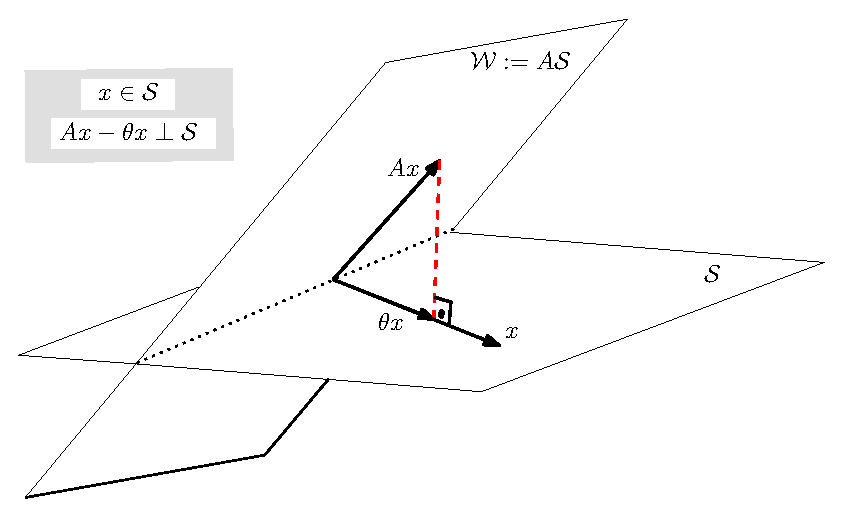
\epsfig{file=alglin_ritzpair,width=0.8\textwidth}
  \caption{Representação esquemática de um par de Ritz.}\label{fig_ritzpair}
\end{figure}

\begin{obs}\label{obs_ritzpair}
Usando a notação da Definição \ref{defi_ritz}, sejam $V\in \mathbb{C}^{m\times n}$  uma matriz cujas colunas são ortonormais ($V^HV=I\in \mathbb{C}^{n\times n}$) e  $\mathcal{S}:=\range{V}$.
 Sejam $\upsilon\in \mathbb{C}^{n}$, $z\in \mathbb{C}^{n}$, $x = V\upsilon$ e $w = Vz$. A equação~\eqref{eq_ritz}
pode ser escrita:
\begin{equation}\label{eq_ritzrepre}
z^H (V^HAV\upsilon - \theta \upsilon) = 0, \forall z\in \mathbb{C}^{n},
\end{equation}
\noindent que se torna um \emph{problema padrão de cálculo de autovalores}

 \begin{equation}\label{eq_rayleighritzritz}
V^HAV\upsilon = \theta\upsilon,
\end{equation}
onde  $x=V\upsilon$, com $\upsilon\in\mathbb{C}^{n}$ e $x\in\mathbb{C}^{m}$, ou seja, $\upsilon$ é  a
representação do vetor de Ritz $x$ na base $\{v_1,v_2,\ldots,v_n\}$.
\end{obs}

A Observação \ref{obs_ritzpair} nos permite fazer uma conexão entre a formulação variacional de Rayleigh-Ritz e o cálculo de um par de Ritz. Da equação \eqref{eq_rayleighritzritz} temos que
\[
\upsilon^HV^HAV\upsilon = \theta\upsilon^H\upsilon\Rightarrow \theta=\frac{\displaystyle x^HAx}{\displaystyle x^Hx}.
\]
Vale insistir que o Teorema \ref{teo_rayrit} tem como hip\'{o}tese a matriz ser hermitiana e essa hip\'{o}tese  não é necessária à definição dos valores de Ritz.

\section{Pares de Ritz harmônicos}\label{sec_parritzharm}

Vamos a uma nova definição, trata-se de uma adaptação do conceito de pares de Ritz para favorecer a análise de certos métodos de Krylov. Neste caso, o vetor harmônico de Ritz será a pré-imagem do vetor de Ritz da inversa de $A$ e o valor harmônico de Ritz será inverso do valor de Ritz da inversa de $A$.

\begin{defi}[Valor Harmônico de Ritz \protect{\cite{PaigeParlettEtAl95Approximate}}]\label{defi_hritz}
 Seja $\mathcal{S}\subset \mathbb{C}^m$. O escalar $\theta\in\mathbb{C}$ é um \textbf{valor harmônico de Ritz} de $A$ em relação um dado espaço $\mathcal{W}\subset \mathbb{C}^m$, caso $\theta^{-1}$ seja um valor de Ritz de $A^{-1}$  com relação $\mathcal{W}:=A\mathcal{S}$.
\end{defi}
Uma representação gráfica para essa definição pode ser vista na Figura \ref{fig_hritzpairorig}.
\begin{figure}[htb]
  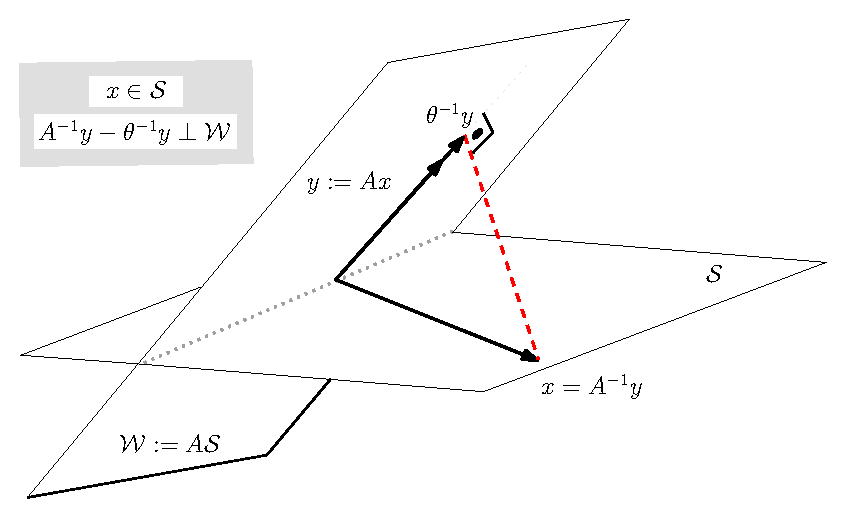
\epsfig{file=alglin_hritzpairorig.eps, width=\textwidth}
  \caption{Representação esquemática de um par harmônico de Ritz usando a representação proposta na Definição \protect{\ref{defi_hritz}}.}\label{fig_hritzpairorig}
\end{figure}
No entanto, usaremos uma outra formulação equivalente, proposta em \cite{SleijpenVorst00JacobiDavidson}, para os valores harmônicos de Ritz.
\begin{teore}[Caracterização dos Pares Harmônicos de Ritz~\protect{\cite[Teorema 5.1, pág. 279]{SleijpenVorst00JacobiDavidson}}]\label{teo_SleijpenVorst00JacobiDavidson}
Sejam $\mathcal{S}\subset \mathbb{C}^m$ e $\mathcal{W}=\{y\in\mathbb{C}^{m};\exists\; x\in S\text{ tal que } y=Ax\}$, ou seja, $\mathcal{W}:=A\mathcal{S}$, então  $\theta\in\mathbb{C}$ é um valor harmônico de Ritz de $A$ em relação a $\mathcal{W}$,  se e somente se,
\begin{equation}\label{eq_hritz}
 w^H(Ax - \theta x) = 0, \forall w \in \mathcal{W},\text{ para algum  }   x\in \mathcal{S},\;x\neq 0.
\end{equation}
Denominaremos $x\in \mathcal{S}$ de \textbf{vetor harmônico de Ritz} associado a $\theta$, e $(x,\theta)\in S\times \mathbb{C}$ de \textbf{par harmônico de Ritz}.  Uma representação gráfica para essa caracterização pode ser vista na figura \ref{fig_hritzpair}.
\end{teore}
\dem
Pelas Definiç\~{o}es em \ref{defi_ritz} e \ref{defi_hritz}, para $\theta$ ser um valor harmônico de Ritz de $A$ em relação à $\mathcal{W}$, existem $y\ne0 \in \mathcal{W}$ e $\theta\in \mathbb{C}$ tais que
\[
 w^H(A^{-1}y - \theta^{-1} y) = 0, \forall w \in \mathcal{W}, y\in\mathcal{W}, y\ne 0.
\]
Basta apenas desenvolver para $y=Ax$, uma vez que  $\mathcal{W}:=A\mathcal{S}$
\[
 w^H(A^{-1}Ax - \theta^{-1} Ax) = 0\Leftrightarrow \theta^{-1}w^H(\theta x - Ax) = 0\Leftrightarrow w^H(\theta x - Ax) = 0.
\]
\fim

\'{E} interessante observar que, no caso real, a equivalência entre as duas formulaç\~{o}es de pares harmônicos de Ritz são simples relaç\~{o}es de semelhança de triângulos retângulos, onde as hipotenusas são $x=A^{-1}y$, com $y \in\mathcal{W},\;y\ne0$,  quando usamos a Definição \ref{defi_hritz}, e $\theta x$, quando lançamos mão da caracterização proveniente do Teorema \ref{teo_SleijpenVorst00JacobiDavidson}, ver Figura \ref{fig_hritzpairtriang}.
\begin{figure}[htb]
  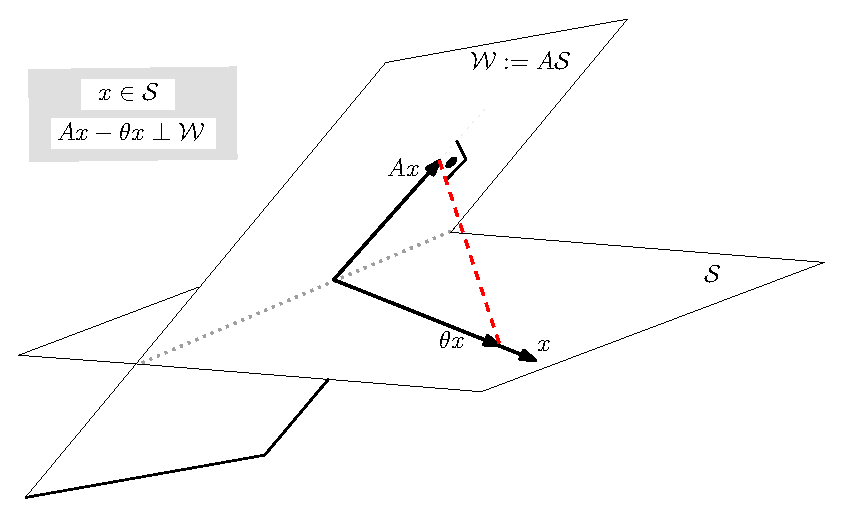
\epsfig{file=alglin_hritzpair.eps, width=\textwidth}
  \caption{Representação esquemática de um par harmônico de Ritz usando a representação proposta no Teorema \protect{\ref{teo_SleijpenVorst00JacobiDavidson}}.}\label{fig_hritzpair}
\end{figure}

\begin{figure}[htb]
  \begin{center}
  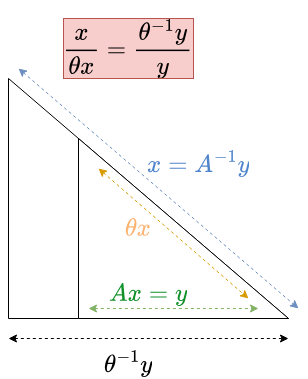
\includegraphics[scale=.7]{triangret.png}
  \caption{ Relações em um triângulo retângulo das representações de um par harmônico de Ritz usando a Definição \protect{\ref{defi_hritz}} e o Teorema \protect{\ref{teo_SleijpenVorst00JacobiDavidson}}. Ver Figuras \protect{\ref{fig_hritzpairorig}} e \protect{\ref{fig_hritzpair}}.}\label{fig_hritzpairtriang}
  \end{center}

\end{figure}
\begin{obs}\label{obs_hritzpair}
Usando a notação do Teorema \ref{teo_SleijpenVorst00JacobiDavidson}, sejam  $V\in \mathbb{C}^{m\times n}$ uma matriz cujas as colunas são ortonormais, $V^HV=I\in \mathbb{C}^{n\times n}$ e
 $\mathcal{S}:=\range{V}$.
Sejam $\chi\in \mathbb{C}^{n}$, $z\in \mathbb{C}^{n}$, $x = V\chi$ e $w = AVz$. A equação~\eqref{eq_hritz}
pode ser escrita como:
\begin{equation}\label{eq_ritzharmorepre}
z^H (V^HA^HAV\chi - \theta V^HA^HV \chi) = 0, \forall z\in \mathbb{C}^{n},
\end{equation}
\noindent levando a um  \emph{problema generalizado de autovalores}:
\begin{equation}\label{eq_hritzgeneigen}
V^HA^HAV\chi = \theta V^HA^HV\chi.
\end{equation}
 Caso $V^HA^HV$ seja uma matriz não singular, esse problema torna-se um problema de autovalores:
\begin{equation}\label{eq_hritzeigen}
\bigg(V^HA^HV\bigg)^{-1}V^HA^HAV\chi = \theta \chi.
\end{equation}
\end{obs}
A Observação \ref{obs_hritzpair} nos permite fazer a conexão entre uma variante da formulação variacional de Rayleigh-Ritz e o cálculo de um par harmônico de Ritz. Senão vejamos: da equação \eqref{eq_hritzgeneigen} temos que
\[
\chi^HV^HA^HAV\chi = \theta \chi^HV^HA^HV\chi\Rightarrow \theta=\frac{\displaystyle (Ax)^HAx}{\displaystyle (Ax)^Hx}.
\]
Aqui, novamente, vale o esclarecimento de que o Teorema \ref{teo_rayrit} tem como hip\'{o}tese a matriz ser hermitiana; hip\'{o}tese desnecessária à definição dos valores harmônicos de Ritz.


Os pares Ritz e os pares harmônicos  Ritz, e algumas de suas variaç\~{o}es \cite{Beattie1998Harmonic}, são bastante utilizados nos métodos iterativos para cálculo de autovalores, ver \cite{BaiDemmelEtAl2000Templates}. Para matrizes hermitianas e para matrizes que não estejam muito longe de serem normais, o comportamento dos autovalores e de suas aproximaç\~{o}es ajudam a compreender o hist\'{o}rico da convergência de alguns  métodos de Krylov \cite{Cullum1996Iterative}, \cite{GreenbaumPtakEtAl96Any}. Com isso, os métodos de Krylov,  quando aplicados à solução de um sistema linear, podem fazer uso de aproximaç\~{o}es de autovalores, que estão implícitas, como veremos a seguir. A princípio, o GMRES com recomeço desconsidera  a maior parte da informação guardada durante a iteração anterior.

O teorema a seguir mostra a transformação do problema de cálculo de pares harmônicos de Ritz apresentado em \eqref{eq_hritzgeneigen} em um  bem mais simples  e demonstra uma propriedade relevante de ortogonalidade dos pares harmônicos de Ritz.

\begin{teore}\label{teo_alglin_arnoldiritz}
Seja $V$ uma matriz cujas as colunas formam uma base ortonormal para $\mathcal{K}^{k+1}(A, r_0)$. Suponhamos que o polinômio mínimo de $r_0$   em relação a $A$ tem grau maior que $k+1$.  Usando a notação do método de Arnoldi a equação para pares harmônicos de Ritz em \eqref{eq_hritzgeneigen} pode ser escrita como

\begin{equation}\label{eq_teo_alglin_arnoldiritzcalcul}
(H_k+h_{(k+1),k}^2 H_k^{-H} e_k e_k^T)\chi =  \theta\chi.
\end{equation}
Seja $(x,\theta)$ um par harmônico de Ritz de A em relação a $A\mathcal{K}_k(A,r_0)$, tal que $x=V_k\chi$, com $\chi\in\mathbb{C}^k$. Então vale a seguinte relação de ortogonalidade:
\begin{equation}\label{eq_teo_alglin_arnoldiritzortho}
\overline{H}_k^H (\overline{H}_k \chi-  \theta\begin{pmatrix} \chi\\0 \end{pmatrix})=0.
\end{equation}

\end{teore}
\dem
\[
   V_k^HA^HAV_k\chi=\theta V_k^HA^HV_k\chi
\]
usando uma das relaç\~{o}es provenientes do método de Arnoldi, $AV_k=V_{k+1}\overline{H}_k$, temos
\[
   \overline{H}_k^H V_{k+1}^HV_{k+1}\overline{H}_k \chi = \theta\overline{H}_k^H V_{k+1}^HV_k\chi
\]
como $V_{k+1}$ é ortogonal, podemos simplificar para
\begin{equation}\label{eq_teo_alglin_arnoldiritzhbarh}
   \overline{H}_k^H\overline{H}_k\chi =\theta\overline{H}_k^H \begin{pmatrix}I_{k\times k}\\ 0\end{pmatrix}\chi
    \Rightarrow
\overline{H}_k^H\overline{H}_k\chi = \theta H_k^H\chi
\end{equation}
escrevendo a matriz $\overline{H}_k$ em blocos, chegamos a
\[
\begin{pmatrix}H_k^H \quad \begin{matrix}0\\\vdots\\0\\h_{(k+1),k} \end{matrix}\end{pmatrix}
 \begin{pmatrix}H_k\\ \begin{matrix}0\;\;\ldots\;\;0\;\;h_{(k+1),k} \end{matrix}\end{pmatrix} =\theta H_k^H\chi
 \]
que pode ser simplificado para
\[(H_k^H H_k+h_{(k+1),k}^2 e_k e_k^T)\chi=\theta H_k^H\chi
\]
como podemos assumir que $H_k$ é não singular, graças à hip\'{o}tese sobre o grau do polinômio mínimo de $r_0$  em relação à $A$, então
\[(H_k+h_{(k+1),k}^2 H_k^{-H} e_k e_k^T)\chi =  \theta\chi.
\]
Provando a relação \eqref{eq_teo_alglin_arnoldiritzcalcul}.

Partindo da equação \eqref{eq_teo_alglin_arnoldiritzhbarh}
\[
  \overline{H}_k^H\overline{H}_k\chi =\theta\overline{H}_k^H \begin{pmatrix}I_{k\times k}\\ 0\end{pmatrix}\chi
\]
com uma simples reorganização, temos
\[
 \overline{H}_k^H (\overline{H}_k \chi-  \theta\begin{pmatrix} \chi\\0 \end{pmatrix})=0.
\]
\fim

 Cabe observar que o teorema anterior está fortemente ancorado no uso do método de Arnoldi para ortogonalização da matriz de Krylov.



O pr\'{o}ximo teorema relaciona os resíduos dos cálculos dos valores harmônicos de Ritz com o resíduo
de uma dada iteração do GMRES, ver \cite{Morgan00Implicitly}.
\begin{teore}\label{teo_alglin_gmresparallel}
Sejam $\overline{H}_k $ e $(\beta e_1-\overline{H}_k y_k)$ provenientes do algoritmo do GMRES e sejam $(x_i,\theta_i)$  pares harmônicos de Ritz de $A$ em relação a $A\mathcal{K}_k(A,r_0)$, tal que $x_i=V_k\chi_i$, com $\chi_i\in\mathbb{C}^k$. Suponhamos que o polinômio mínimo de $r_0$   em relação a $A$ tem grau maior que $k+1$. Então


\begin{equation}\label{eq_arnolditeo3}
\overline{H}_k \chi_i -\theta_i\begin{pmatrix} \chi_i\\0 \end{pmatrix}=
\alpha_i(\beta e_1-\overline{H}_k y_k),
\end{equation}
com $\alpha_i$ escalares.
\end{teore}
\dem
Pelo resultado encontrado em \cite[corolário 1.39 do teorema 1.38, pág. 36]{Saad03Iterative}, temos que $\beta e_1-\overline{H}_k y_k$
é ortogonal a  $\overline{H}_k y,\;\forall y\in\mathbb{C}^k$, onde
\[
y_k= \arg\underset{y\in\mathbb{C}^k}{\min}
\Vert \beta e_1-\overline{H}_k y\Vert_2.
\] Então
\[
(\beta e_1-\overline{H}_k y_k)\perp \range{\overline{H}_k}.
\]
 Usando \eqref{eq_teo_alglin_arnoldiritzortho}, podemos escrever que
\[
(\overline{H}_k \chi_i -\theta_i\begin{pmatrix} \chi_i\\0 \end{pmatrix}) \perp \range{\overline{H}_k}
.\]
Logo ambos os vetores pertencem ao $\Ker{\overline{H}_k}$, mas pela hip\'{o}tese sobre o grau do polinômio mínimo de $r_0$ em relação a $A$, $H_k$ tem posto completo,
$\Ker{\overline{H}_k}$ tem dimensão 1, e
\[(\beta e_1-\overline{H}_k y_k) \text{ é paralelo a }
(\overline{H}_k \chi_i -\lambda_i\begin{pmatrix} \chi_i\\0 \end{pmatrix}).
\]
\fim





%
\markboth{}{Bibliografia}

\begin{thebibliography}{100}
	
    \bibitem{Arnoldi51principle} W.~E. Arnoldi. \newblock The principle of minimized iterations in the solution of the
    matrix
  eigenvalue problem.
\newblock {\em Quart. of Appl. Math.}, 9(1):17--29, 1951.


	\bibitem{BaiDemmelEtAl2000Templates} Z.~Bai, J.~Demmel, J.~Dongarra, A.~Ruhe, and H.~van~der Vorst, editors.
	\newblock {\em Templates for the solution of Algebraic Eigenvalue Problems: A
		Practical Guide}.
	\newblock SIAM, Philadelphia, 2000.


	\bibitem{Beattie1998Harmonic} C.~Beattie. \newblock Harmonic {R}itz and {L}ehman bounds. \newblock {\em ETNA},
	7:18--39, 1998.

	\bibitem{Brezinski2002Outils} C.~Brezinski. \newblock {\em Outils d'analyse numérique pour l'automatique},
    chapter
  Résolution des systèmes linéaires, pages 109--144.
\newblock Hermes Science Publications, 2002.

\bibitem{Chaitin-ChatelinFraysse1996Lectures} F.~{Chaitin-Chatelin} and V.~Frayssé. \newblock {\em Lectures on
    Finite Precision Computations}. \newblock SIAM, Philadelphia, 1996.



	\bibitem{Cullum1996Iterative} J.~K. Cullum. \newblock Iterative methods for solving ${A}x=b$ {GMRES-FOM} versus
	{QMR/BiCG}. \newblock Technical Report TR-96-2, Institute for Advances Studies, University
	of Maryland, 1996.
	
	\bibitem{Embree1999How} M.~Embree. \newblock How descriptive are {GMRES} convergence bounds? \newblock Technical
report, Oxford University Computing Laboratory, 1999.

	\bibitem{GoossensRoose99Ritz} S.~Goossens and D.~Roose. \newblock {Ritz} and harmonic {Ritz} values and the
	convergence of {FOM} and
	{GMRES}.
	\newblock {\em Numerical linear algebra with applications}, 6(4):281--293,
	1999.
	
	\bibitem{Greenbaum97Iterative} A.~Greenbaum. \newblock {\em Iterative Methods for Solving Linear Systems}.
    \newblock SIAM, Philadelphia, 1997.
	
	
	\bibitem{GreenbaumPtakEtAl96Any} A.~Greenbaum, V.~Pták, and Z.~Strako{\u{s}}. \newblock Any nonincreasing
	convergence curve is possible for {GMRES}. \newblock {\em SIAM Journal on Matrix Analysis and Applications},
	17(3):465--469, July 1996.
	

	

	
	\bibitem{HornJohnson1985} R.A.~Horn and C.R~Johnson. \newblock {\em Matrix Analysis}. \newblock
	Cambridge University Press, 1985.
  
  
	

		
	\bibitem{HornJohnson87Matrix} R.~A. Horn and C.~R. Johnson. \newblock {\em Matrix Analysis}. \newblock Cambridge
	University Press, 1987.
	


	
	\bibitem{JiaStewart2001analysis} Z.~Jia and G.~W. Stewart. \newblock An analysis of the {Rayleigh-Ritz} method for
	approximating
	eigenspaces.
	\newblock {\em Mathematics of Computation}, 70(234):637--647, 2001.
	
	\bibitem{Meurant1999Computer} G.~Meurant. \newblock {\em Computer solution of large linear systems}. \newblock
    North-Holland, 1999.

    \bibitem{Meurant2020Krylov}  G.~Meurant and J.D.~Tebbens.
    \newblock{\em Krylov Methods for Nonsymmetric Linear Systems}, Springer, 2020.
	

	

	
	\bibitem{Meyer00Matrix} C.~D. Meyer. \newblock {\em Matrix analysis and applied liner algebra}. \newblock SIAM,
	2000.
	
\bibitem{Morgan1991Computing} R.~B. Morgan. \newblock Computing interior eigenvalues of large matrices. \newblock
{\em Lin. Alg. and Its Applic.}, 154/156:289--309, 1991.

\bibitem{Morgan95Restarted} R.~B. Morgan. \newblock A restarted {GMRES} method augmented with eigenvectors.
    \newblock {\em SIAM Journal on Matrix Analysis and Applications},
  16(4):1154--1171, 1995.


\bibitem{Morgan00Implicitly} R.~B. Morgan. \newblock Implicitly restarted {GMRES} and {Arnoldi} methods for
nonsymmetric
systems of equations.
\newblock {\em SIAM Journal on Matrix Analysis and Applications},
21(4):1112--1135, 2000.
	
\bibitem{NachtigalReddyEtAl1992How} N.~M. Nachtigal, S.~C. Reddy, and L.~N. Trefethen. \newblock How fast are
    nonsymmetric matrix iterations? \newblock {\em SIAM Journal on Matrix Analysis and Applications},
  13(3):778--795, 1992.

  \bibitem{PaigeParlettEtAl95Approximate} C.~C. Paige, B.~N. Parlett, and H.~A. van~der Vorst. \newblock Approximate
  solutions and eigenvalue bounds from {Krylov} subspaces. \newblock {\em Numerical Linear Algebra with
  Applications}, 2(2):115 -- 133,
1995.

\bibitem{PaigeRozloznikEtAl2006MODIFIED} C.~C. Paige, M.~Rozlo{\u{z}}n{\'{\i}}k, and Z.~Strako{\u{s}}. \newblock
  Modified {G}ram-{S}chmidt ({MGS}), least squares, and backward
stability of {MGS-GMRES}.
\newblock {\em SIAM Journal on Matrix Analysis and Applications},
28(1):264--284, 2006.


	
	\bibitem{Parlett1998symmetric} B.~N. Parlett. \newblock {\em The symmetric eigenvalue problem}. \newblock SIAM,
	Philadelphia, 1998. \newblock Corrected reprint of the 1980 original.

\bibitem{Rozloznik1997Numerical} M.~Rozlo\u{z}ník. \newblock {\em Numerical Stability of the GMRES Method}.
    \newblock PhD thesis, Institute of Computer Science, Academy of Sciences of the
  Czech Republic, Prague, April 1997.


\bibitem{Saad1981Krylov} Y.~Saad. \newblock {Krylov} subspace methods for solving large unsymmetric linear
  systems.
\newblock {\em Math. Comp.}, 37(155):105--126, July 1981.

	\bibitem{Saad03Iterative} Y.~Saad. \newblock {\em Iterative Methods for Sparse Linear Systems}. \newblock SIAM,
	2nd edition, 2003.
	
	\bibitem{SaadSchultz86GMRES} Y.~Saad and M.~H. Schultz. \newblock {GMRES}: a generalized minimal residual
    algorithm for solving
  nonsymmetric linear systems.

  \bibitem{SaadVorst00Iterative} Y.~Saad and H.~A. van~der Vorst. \newblock Iterative solution of linear systems in
    the 20th century. \newblock {\em Journal of Computational and Applied Mathematics},
  123(1-2):1--23, 2000.



	
	\bibitem{Scott1982Advantages} D.~S. Scott. \newblock The advantages of inverted operators in {Rayleigh--Ritz}
	approximations.
	\newblock {\em SIAM Journal on Scientific and Statistical Computing},
	3(1):68--75, 1982.
		
	\bibitem{Simoncini00Convergence} V.~Simoncini. \newblock On the convergence of restarted {Krylov} subspace
    methods. \newblock {\em SIAM Journal on Matrix Analysis and Applications},
  22(2):430--452, 2000.

 
    \bibitem{SimonciniSzyld2007Recent} V.~Simoncini and D.~B. Szyld. \newblock Recent computational developments in
    {Krylov} subspace methods for
  linear systems.
\newblock {\em Numerical Linear Algebra with Applications}, 14:1 -- 59, 2007.

		
	\bibitem{SleijpenEshof2003use} G.~L.~G. Sleijpen and J.~van~den Eshof. \newblock On the use of harmonic {Ritz}
	pairs in approximating internal
	eigenpairs.
	\newblock {\em Linear Algebra and its Applications}, 358(1-3):115--137, January
	2003.
	
	\bibitem{SleijpenVorst00JacobiDavidson} G.~L.~G. Sleijpen and H.~A. van~der Vorst. \newblock A {Jacobi--Davidson}
	iteration method for linear eigenvalue problems. \newblock {\em SIAM Review}, 42(2):267--293, 2000. \newblock
	This paper originally appeared in SIAM Journal on Matrix Analysis and
	Applications, Volume 17, Number 2, 1996, pages 401-425.
	

	\bibitem{Stewart1973Introduction} G.~W. Stewart. \newblock {\em Introduction to Matrix Computations}. \newblock
    Academic Press, New York, 1973.

    \bibitem{Stewart98Matrix} G.~W. Stewart. \newblock {\em Matrix Algorithms. {Volume I}: Basic Algorithms}.
    \newblock SIAM, Philadelphia, PA, USA, 1998.


	
	\bibitem{Stewart01Matrix} G.~W. Stewart. \newblock {\em Matrix Algorithms. {Volume II}: Eigensystems}. \newblock
	SIAM, 2001.
	
	
	\bibitem{Trefethen1990Algorithms} L.~N. Trefethen. \newblock {\em Algorithms for Approximation II}, chapter
    Approximation theory
  and numerical linear algebra, pages 336--360.
\newblock Chapman and Hall, London, 1990.


	
	
\bibitem{Vorst03Iterative} H.~van~der Vorst. \newblock {\em Iterative {Krylov} Methods for Large Linear systems}.
\newblock Cambridge University Press, Cambridge, April 2003.
	
	
\bibitem{Zemke2003Krylov} J.-P.~M. Zemke. \newblock {\em {Krylov} Subspace Methods in Finite Precision: A Unified
Approach}.
\newblock PhD thesis, Technischen Universität Hamburg-Harburg, 2003.
	
	
\bibitem{Zou2023}  Q. Zou.
\newblock  {GMRES} algorithms over 35 years,
   \newblock{\em Applied Mathematics and Computation},
 2023.
			

	
	
	\markboth{}{}
	
\end{thebibliography}



\bibliographystyle{plain} 
\bibliography{krylov.bib}

\end{document}
